\chapter{Zapoznanie z~alokatorem stron}

Ponieważ mechanizm CMA w~dużym stopniu integruje się z~podsystemem
zarządzania pamięci (\ang{memory management} lub w~skrócie mm), do
jego zrozumienia potrzeba ogólnej wiedzy na temat tego w~jaki sposób
jądro śledzi i~przydziela pamięć procesom i~sterownikom.

Linux posiada wiele mechanizmów alokacji pamięci.  Począwszy od
najprostszych w~użyciu funkcji \code|kmalloc| i \code|vmalloc|,
poprzez mechanizmy puli pamięci, aż do alokatora czasu bootowania
i~alokatorów pamięci dostępnej dla urządzeń zewnętrznych
\autocite[rozdział 8]{bib:ldd3}.  Pomimo tak dużej liczby interfejsów,
wiele z~nich sprowadza się do wywołania alokatora stron (\ang{page
  allocator}), który jest sercem podsystemu zarządzania pamięcią.
Uproszczone zależności między tymi komponentami przedstawia rysunek
\ref{fig:allocators-base}.

\section{Algorytm bliźniaków}

Alokator stron implementuje algorytm bliźniaków (skąd też jego inna
angielska nazwa: {\it buddy system} lub {\it buddy allocator}), który
operuje na blakach o~rozmiarze $2^k$ jednostek.  W~przypadku Linuksa
jednostką jest pojedyncza strona fizyczna, a~na $k$~narzucone jest
ograniczenie $k < \mathrm{MAX\_ORDER}$.  \code|MAX_ORDER| może
zależeć od architektury, na którą Linux jest kompilowany, ale
zazwyczaj ma wartość $11$ (toteż na potrzeby tej pracy zakładam, iż $0
\le k \le 10$).

\begin{wrapfigure}{o}[1.5cm]{0.3\textwidth}
\begin{center}
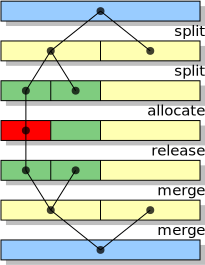
\includegraphics[width=0.25\textwidth]{build/alloc-free-cycle.eps}
\end{center}
\caption[Zarządzanie pamięcią w~algorytmie bliźniaków]{Graficzna
  reprezentacja cyklu alokacji i~zwalniania buforów w~algorytmie
  bliźniaków.}
\end{wrapfigure}

W~Linuksie, przez $k$ rozumie się rząd strony (\ang{page order}).
Strona rzędu 0 to pojedyncza strona fizyczna, strona rzędu 1
(\ang{1-order page}) to dwie strony fizyczne itd.\ aż do strony rzędu
10, czy też strony maksymalnego rzędu (\ang{max order page}), która
składa się z~1024 stron fizycznych.  Ogólnie, strona rzędu $n$ składa
się z~dwóch stron rzędu $n-1$.

Funkcja \code|alloc_pages|, która jest interfejsem dla alokatora
stron, przyjmuje jako argument właśnie rząd żądanej strony.  Wynikają
stąd następujące właściwości alokatora stron:

\begin{itemize}
\item Nie można za jego pomocą zaalokować mniej niż jednej strony,
  tj.\ 4096 bajtów.
\item Interfejs nie pozwala alokować obszarów, których rozmiar nie
  jest potęgą dwójki.
\item Gdyby jednak chcieć zaalokować taki obszar, wiązałoby się to
  z~potencjalnie dużą fragmentacją wewnętrzną.  Dla przykładu kolorowa
  tekstura o~rozmiarze $512 \times 512$ pikseli zajmuje
  \unit[768]{KiB}, zatem bufor ją przechowujący musiałby mieć rozmiar
  \unit[1]{MiB}, z~których \unit[256]{KiB}, a~więc \nicefrac{1}{4},
  byłoby nieużywane.
\item Alokator stron nie jest w~stanie zaalokować obszaru większego
  niż \unit[4]{MiB}.  Z~tego powodu, nie nadaje się do alokowania
  ciągłego fizycznie buforu dla pięciomegapikselowej kamery, czy nawet
  pojedynczej ramki {\it full HD}.
\end{itemize}

\begin{figure}[tbp]
  \centering
  \includegraphics[width=\textwidth]{build/linux-allocators--base.eps}
  \caption[Alokatory dostępne w~jądrze Linux.]{Relacje między kilkoma
    najistotniejszymi alokatorami pamięci dostępnymi w~Linuksie.}
  \label{fig:allocators-base}
\end{figure}

Jak zatem działa algorytm bliźniaków?  Alokator posiada listę wolnych
stron, których rząd jest pomiędzy $0$ a~$10$.  W~Linuksie zrealizowane
jest to poprzez 11 list dwukierunkowych, gdzie każda przeznaczona jest
dla stron o~konkretnym rzędzie.

Gdy sterownik chce zaalokować stronę rzędu $n$, alokator sprawdza
odpowiednią listę.  Jeżeli jest ona pusta, przechodzi do listy ze
stronami rzędu $n+1$, aż znajdzie wolną stronę (lub dojdzie do
maksymalnego rzędu, co sygnalizuje nieudaną alokację.  Jeżeli uzyskana
w~ten sposób strona ma rząd większy niż żądany, jest ona dzielona na
pół, aż do osiągnięcia żądanego rozmiaru.  Strony, które powstały na
skutek podziału większej strony na pół, nazywamy stronami
bliźniaczymi.  Cały proces ilustruje algorytm \ref{alg:buddy-alloc}

\begin{algorithm}
\caption[Alokacja strony w~algorytmie bliźniaków.]{Alokacja strony
  rzędu $k$ w~algorytmie bliźniaków.}
\label{alg:buddy-alloc}
\begin{algorithmic}[1]
\Require $0 \leq k < \mathrm{MAX\_ORDER}$
\Function{AllocatePage}{$k$}
    \State $i \gets k$
    \While {lista stron rzędu $i = \emptyset$}
        \State $i \gets i + 1$
        \If {$i = \mathrm{MAX\_ORDER}$}
            \State \Return $\emptyset$
        \EndIf
    \EndWhile

    \State $p \gets$ strona z listy stron rzędu $i$
    \While {$i \neq k$}
        \State $i \gets i - 1$
        \State podziel $p$ na pół na $p_1$ i $p_2$
        \Comment{Strony $p_1$ i $p_2$ nazywamy stronami bliźniaczymi}
        \State $p \gets p_1$
        \State dodaj $p_2$ do listy stron rzędu $i$
    \EndWhile
    \State \Return $p$
\EndFunction
\end{algorithmic}
\end{algorithm}

Przy zwalnianiu, dopóki to możliwe, strona jest łączona ze swoją
bliźniaczą stroną, dzięki czemu strony są dodawane do listy wolnych
stron o~dużym rzędzie.  Proces ten ilustruje algorytm
\ref{alg:buddy-free}

\begin{algorithm}
\caption[Zwalnianie strony w~algorytmie bliźniaków.]{Zwalnianie strony
  $p$ rzędu $k$ w algorytmie bliźniaków.}
\label{alg:buddy-free}
\begin{algorithmic}[1]
\Procedure{FreePage}{$p$, $k$}
    \While {$k + 1 \neq \mathrm{MAX\_ORDER} \wedge p$ posiada wolną stronę bliźniaczą}
        \State $p' \gets$ strona bliźniacza $p$
        \State usuń $p'$ z~listy wolnych stron
        \State $k \gets k + 1$
        \State $p~\gets$ strona powstała w~wyniku połączenia $p$ i~$p'$ \label{alg:buddy-free:join}
    \EndWhile
    \State dodaj $p$ do listy wolnych stron rzędu $k$ \label{alg:buddy-free:add}
\EndProcedure
\end{algorithmic}
\end{algorithm}

Dokładniejszy opis algorytmu bliźniaków oraz przedstawienie jego
właściwości można znaleźć na stronach 435--455
\autocite{bib:taocp-fa}, a~jego zastosowanie w~Linuksie w~podrozdziale
8.1.7 \autocite{bib:utlk}.


\section{Migracja i~typy migracji}\label{sec:migratetype}

Kolejnym istotnym elementem alokatora stron pominiętym z~opisu
w~poprzednim podrozdziale są typy migracji (\ang{migratetype}),
których jest sześć: {\it unmovable}, {\it reclaimable}, {\it movable},
{\it cma}, {\it reserve} oraz {\it isolate}).

\begin{itemize}
\item Dla potrzeb tej pracy traktuję typy {\it unmovable}, {\it
  reclaimable} i~{\it reserve} jak jeden typ -- typ nieruchomy.  To
  uproszczenie wynika z~faktu, iż dla mechanizmu CMA istotne jest
  tylko rozróżnienie pomiędzy stronami ruchomymi i~nieruchomymi.
\item Strony które są typu ruchomego charakteryzują się tym, że ich
  adres fizyczny nie jest istotny, w~związku z~czym mogą być
  przeniesione w~inne miejsce pamięci RAM.
\item Typ {\it cma} jest nowym typem dodanym dla potrzeb interfejsu
  CMA i~jest opisany dokładniej w~podrozdziale \ref{sec:migrate-cma}.
\item Typ {\it isolate} jest niejako pseudo-typem, gdyż jeżeli wolna
  strona ma taki typ, nie może ona zostać zaalokowana.  Więcej na
  temat sposobu w~jaki ten typ może być wykorzystywany opisuję
  w~podrozdziale \ref{sec:alloc-contig-range}.
\end{itemize}

Jednym z~przykładów stron ruchomych są strony anonimowe działających
procesów.  Ponieważ program odwołują się do nich poprzez mapowania
wirtualne, o~ile tablice translacji zostaną uaktualnione, zawartość
strony może być przeniesiona w~dowolne inne miejsce.  Podobnie wygląda
sprawa z~buforami dyskowymi i~wieloma innymi strukturami, którymi
zarządza jądro.

Proces przenoszenia ruchomej strony nazywa się migracją
i wykorzystywany jest między innymi przy obsłudze hot-swapu pamięci,
a~także w~trackie procesu zagęszczania \autocite{bib:compaction,
  bib:supporting-large-contig-regions}, którego celem jest zwiększenie
liczby dostępnych stron o~wysokich rzędach.

\begin{algorithm}
\caption[Migracja strony.]{Migracja strony $p$.}
\label{alg:migrate}
\begin{algorithmic}[1]
\Procedure{MigratePage}{$p$}
    \State $p' \gets$ \Call{AllocPage}{$0$}
    \State skopiuj zawartość $p$ do $p'$
    \State uaktualnij odwołania do $p$ tak aby wskazywały na $p'$
    \State \Call{FreePage}{$p$, $0$}
\EndProcedure
\end{algorithmic}
\end{algorithm}

Najbardziej skomplikowanym krokiem migracji -- zilustrowanej poprzez
algorytm \ref{alg:migrate} -- jest uaktualnienie odwołań do strony
tak, aby wskazywały na nową stronę $p'$.  Ponieważ istnieje wiele
rodzajów stron ruchomych (strony anonimowe, bufory dyskowe itp.), jest
to krok specyficzny dla danej strony.

Przykładowo dla stron anonimowych wiąże się to z~uaktualnieniem
tablicy translacji adresów tak, aby wskazywały w~nowe miejsce, a~także
wyczyszczeniem pamięci TLB (\ang{Translate Lookaside Buffer}), aby nie
posiadała, żadnych nieaktualnych wpisów.

Wołając funkcję \code|alloc_pages|, typ migracji strony jest
przekazywany jako argument, co pozwala alokatorowi stron grupować
strony tego samego typu.  Jest to istotne, gdyż mechanizm zagęszczania
nie działa zbyt dobrze jeżeli ruchome strony przelatają się
z~pozostałymi stronami, które nie podlegają migracji.


\section{Grupy stron}

Grupowanie stron realizowane jest poprzez podział pamięci na bloki
(\ang{pageblock}) składające się z~\code|pageblock_nr_pages| stron
(czy też równoważnie na bloki rzędu \code|pageblock_order|).
Konkretne wartości tych stałych zależą od architektury, no którą jądro
zostało skompilowane, jak i~opcji konfiguracyjnych wybranych w~trakcie
kompilacji.  Niemniej przeważnie wartość tych stałych to odpowiednio
1024 (stron) i~(rząd) 10 i~właśnie takie są przyjęte w~tej pracy
i~wykorzystane w~graficznej reprezentacji na rysunku \ref{fig:pages}.

\begin{figure}[tbp]
\begin{center}
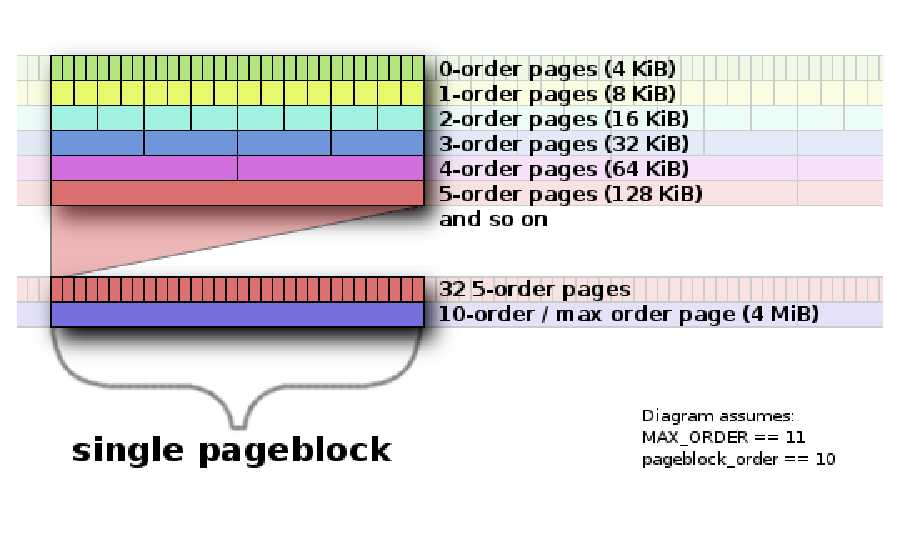
\includegraphics[width=0.8\textwidth]{build/pages.eps}
\end{center}
\caption[Organizacja pamięci w~Linuksie.]{Graficzna reprezentacja
  organizacji stron pamięci stosowanej w~podsystemie zarządzania
  pamięcią Linuksa.}
\label{fig:pages}
\end{figure}

Każdy blok stron (\ang{pageblock}) ma przypisany typ migracji,
a~alokator stron posiada oddzielne listy wolnych stron dla każdego
typu migracji.  Zatem patrząc na algorytm \ref{alg:buddy-alloc} należy
zdawać sobie sprawę, iż rozpatruje on listy wolnych stron danego typu
migracji.

\section{Zmiana typu migracji}\label{sec:type-change}

Należy pamiętać, iż dla jądra zrealizowanie alokacji jest ważniejsze
od trzymania stron o~tym samym typie migracji razem.  Dlatego dla
każdego typu migracji istnieje lista zapasowych (\ang{fallback}) typów
migracji.  Jeżeli alokacja dla żądanego typu migracji nie powiedzie
się, alokator stron będzie próbował z~kolejnymi typami z~list, tak jak
to pokazuje algorytm \ref{alg:buddy-fallback}

Co więcej, jeżeli rząd żądanej strony jest dostatecznie duży, typ
migracji wszystkich wolnych stron w~danym bloku zostaje zmieniano na
ten zgodny z~wywołaniem funkcji \code|alloc_pages|.

\begin{algorithm}
\caption[Alokacja z~uwzględnieniem typu migracji.]{Alokacja strony
  rzędu $k$ z~uwzględnieniem typu migracji $m$}
\label{alg:buddy-fallback}
\begin{algorithmic}[1]
\Function{ChangeBlockMigrateType}{$b$, $m$}
\State zmień typ migracji $b$ na $m$
\ForAll {wolnych stron $p' \in b$}
    \State przenieś $p'$ na listę wolnych stron typu $m$
\EndFor
\EndFunction
\Statex
\Function{AllocPageMigrateType}{$k$, $m$}
    \State $f \gets$ lista zapasowych typów migracji dla typu $m$
    \State dodaj $m$ na początek $f$
    \ForAll{$m' \in f$}
        \State $p \gets$ \Call{AllocPage}{$k$} biorąc pod uwagę listy stron typu $m'$
        \If {$p \neq \emptyset$}
            \If {$m \neq m' \wedge k \geq \nicefrac{\mathrm{page\_order}}{2}$}
                \State $b \gets$ blok stron zawierający $p$
                \State \Call{ChangeBlockMigrateType}{$b$, $m$}
            \EndIf
            \State \Return $p$
        \EndIf
    \EndFor
    \State \Return $\emptyset$
\EndFunction
\end{algorithmic}
\end{algorithm}

Podczas zwalniania, gdy strona jest dodawana do listy wolnych stron
(wideczne w~linii \ref{alg:buddy-free:add} algorytmu
\ref{alg:buddy-free}) typ migracji listy, na którą strona trafia
determinowany jest poprzez typ migracji przypisany blokowi stron do
którego dana strona należy.

Istotne jest tutaj, aby zauważyć, iż bloki stron mogą zmieniać swój
typ migracji, a~także, że nawet jeżeli blok ma dany typ migracji,
strony o~innym typie migracji mogą być z~niego przydzielone.


\section{Listy PCP}\label{sec:pcp-lists}

Ostatnim istotnym, z~punktu widzenia mechanizmu CMA, aspektem
alokatora stron są listy PCP (\ang{per CPU pages})
\autocite[podrozdział 8.1.8]{bib:utlk}.  Ponieważ listy wolnych stron
są współdzielone w~obrębie całego systemu dostęp do nich musi być
synchronizowany pomiędzy wszystkimi procesorami.  Aby uniknąć kosztów
związanych z~synchronizacją, każdy procesor posiada swoje prywatne
listy PCP, na których znajdują się wolne strony rzędu 0.  Biorąc
również i~ten aspekt pod uwagę, alokacja przyjmuje postać
przedstawianą w~algorytmie \ref{alg:buddy-pcp}

\begin{algorithm}
\caption[Alokacja z~uwzględnieniem list PCP.]{Alokacja strony rzędu
  $k$ z~typem migracji $m$ z~uwzględnieniem list PCP.}
\label{alg:buddy-pcp}
\begin{algorithmic}[1]
\Function{AllocPageUsePCP}{$k$, $m$}
    \If {$k \neq 0$}
        \State $p \gets$ \Call{AllocPageMigrateType}{$k$, $m$}
    \Else
        \State $l \gets$ lista PCP dla typu migracji $m$
        \If {$l = \emptyset$}
            \State $i \gets 0$
            \Repeat
                \State $p \gets$ \Call{AllocPageMigrateType}{$0$, $m$}
                \If {$p \neq \emptyset$}
                    \State dodaj $p$ do $l$
                    \State $i \gets i + 1$
                \EndIf
            \Until {$i \geq n \vee p = \emptyset$} \Comment{Wartość
              $n$ jest zależna od różnych czynników}
        \EndIf
        \If {$l = \emptyset$}
            \State \Return $\emptyset$
        \Else
            \State $p \gets$ pierwsza strona z $l$
            \State usuń pierwszą stronę z $l$
            \State lista PCP dla typu migracji $m$ $\gets l$
        \EndIf
    \EndIf
    \State \Return $p$
\EndFunction
\end{algorithmic}
\end{algorithm}


\section{Inne aspekty alokatora stron}

Powyższy opis pomija wiele szczegółów alokatora stron, które nie są
istotne z~punktu widzenia mechanizmu CMA.  Niemniej dla porządku
wymienię kilka istotniejszych detali, które wpływają w~dużej mierze na
sposób w~jaki Linux zarządza pamięcią.

Po pierwsze cała pamięć podzielona jest na strefy (\ang{zones})
\autocite[podrozdział 8.1.3]{bib:utlk}, których, zależnie od
architektury oraz opcji kompilacji, może być pięć:

\begin{description}
\item[ZONE\_DMA] Strefa przeznaczona dla urządzeń, które nie są
  w~stanie wykonywać transferów DMA w~całej przestrzeni adresowej.  Na
  przykład w~architekturze x86 strefa ta jest przeznaczona dla
  urządzeń ISA, które operują na 24-bitowy adresach.
\item[ZONE\_DMA32] Strefa przeznaczona dla urządzeń operujących
  na 32-bitowych adresach pracujących w~architekturze x86\_64.
\item[ZONE\_NORMAL] Strefa z~„normalnymi” stronami, które są na
  stałe zmapowane w~przestrzeni adresowej jądra.
\item[ZONE\_HIGHMEM] Strefa ze stronami, dla których zabrakło
  adresów logicznych w~przestrzeni jądra i~które nie posiadają stałego
  mapowania.
\item[ZONE\_MOVABLE] Strefa, z~które można alokować jedynie
  strony ruchome.
\end{description}

Co więcej, pamięć jest również podzielona na węzły (\ang{nodes}),
które odpowiadają wezłom w~systemach z~niejednolitym dostępem do
pamięci (\ang{Non-Uniform Memory Access} lub NUMA)
\autocite[podrozdział 8.1.2]{bib:utlk}.  Ponieważ w~architekturach
tego typu czas dostępu do pamięci zależy od jej miejsca względem
procesora, istotne jest alokowanie buforów blisko procesora, który
bódzie z~nich korzystał.

Niniejszy rozdział przemilczał również co się dzieje jeżeli podczas
alokacji wolna pamięć nie może zostać odnaleziona.  Otóż jeżeli
algorytm \ref{alg:buddy-alloc} nie znajdzie żadnej wolnej strony
aktywowana jest tzw.\ wolna ścieżka (\ang{slow path}), która
wykorzystuje różne mechanizmy odzyskiwania pamięci (np.\ poprzez
zwalnianie buforów dyskowych, czy w~najgorszym przypadku zabiciu
jednego z~działających procesów, czego dokonuje {\it out-of-memory
  killer} lub OOM {\it killer}) \autocite[rozdział 17]{bib:utlk}.

Istnieje jeszcze wiele innych aspektów takich -- jak chociażby
alokacja w~kontekście atomowym (np.\ w~trakcie obsługi przerwania),
tzw.\ wskaźniki poziamu wody (\ang{watermarks}), które kontrolują jak
duży wolnej pamięci jest w~systemie -- które wprowadzają dodatkową
komplikację do podsystemu zarządzania pamięcią, jednak ponieważ nie
mają one wpływu na mechanizm CMA, wychodzą poza zakres niniejszej
pracy w~związku z~czym są całkowicie ignorowane.
